%! tex root = ../master.tex

\newcommand{\excreturn}{EXC\_RETURN}

\chapter{System Implementation}
{INTRO, to be reviewed}
This chapter deals with how the system\textquotesingle s functionalities 
are implemented. Diagrams will be included when necessary, as well as code 
snippets for the interesting parts of the program. In the end, all these
will be reviewed and compared with the actual requirements of the standard.


\section{Hardware}

As mentioned in the previous chapter, the hardware used for this project 
is a MINI-M4 board from MikroElectronica. This is build around an
STM32F415RG microcontroller produced by STMicroelectronics. Besides
this, the board contains two crystal oscillators, two LEDs, a reset 
button and the peripherals for supplying power via a microUSB connector.
Some of the GPIOs are break through using external pins.
These pins were soldered to the board, and this was setup on a breadboard
for practicality, as seen in \ref{fig:photo1}.

\begin{figure}[H]
\begin{subfigure}{0.5\textwidth}
  \centering
  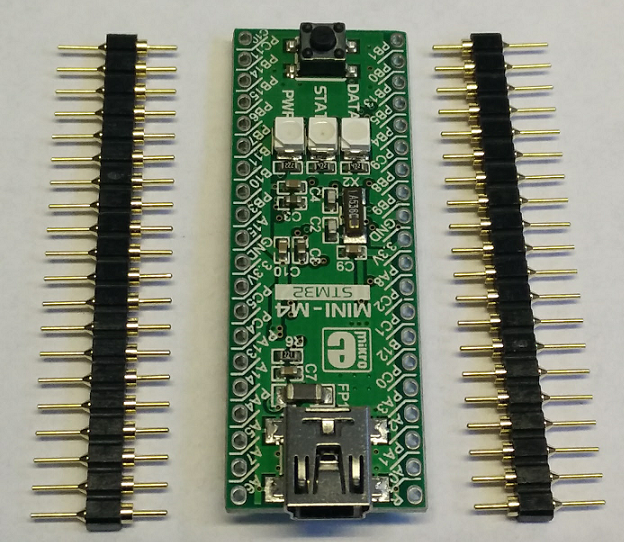
\includegraphics[width=3cm]{hardware/board_not_soldered.png}
  \caption{MINI-M4 before soldernig}
  \label{fig:sub1}
\end{subfigure}%
\begin{subfigure}{0.5\textwidth}
  \centering
  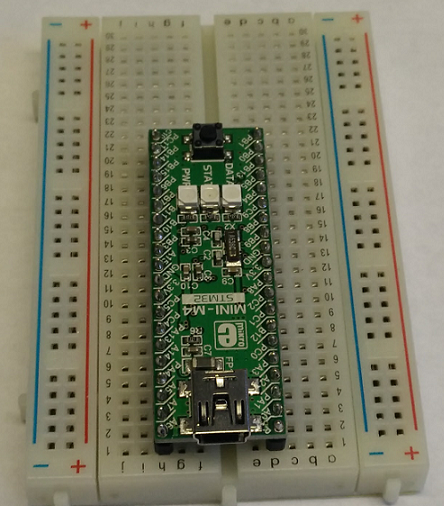
\includegraphics[width=3cm]{hardware/board_on_breadboard.png}
  \caption{MINI-M4 on a breadboard}
  \label{fig:sub2}
\end{subfigure}
\caption{Preparation of the board}
\label{fig:photo1}
\end{figure}

For programming and debugging the board the JTAG interface was used.
This had to be connected to certain pins of the board. In order to get 
feedback from the board, a serial connection was used, which requires two
more lines to it. The final setup can be seen in the next figures.

\begin{figure}[H]
\centering
\begin{subfigure}{.5\textwidth}
  \centering
  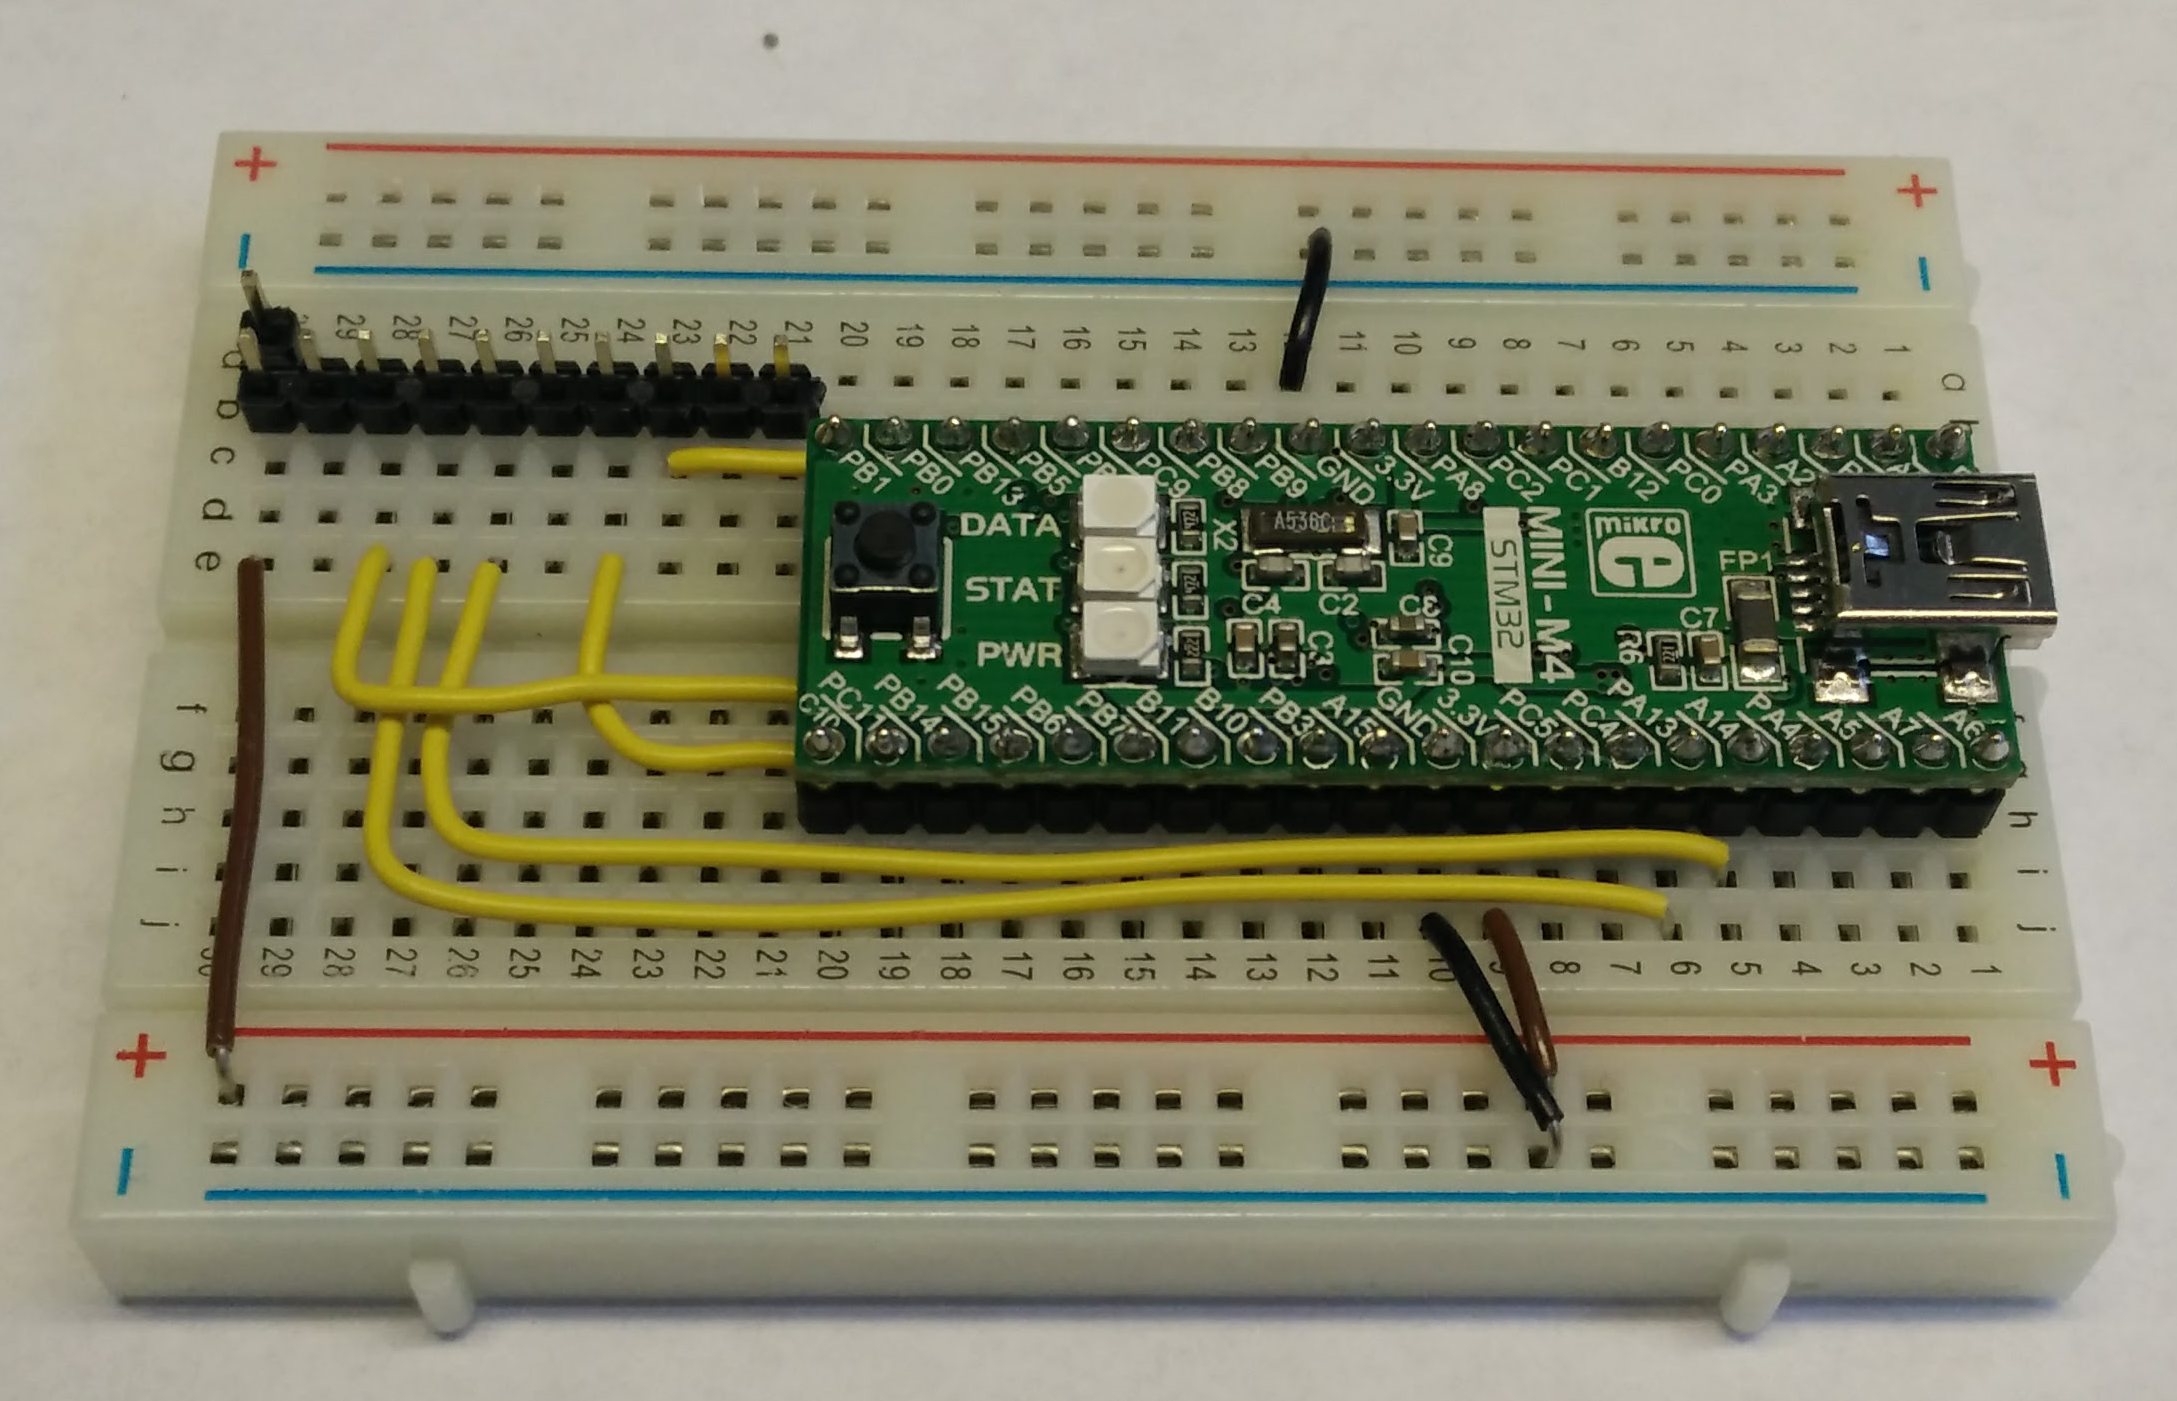
\includegraphics[width=.4\linewidth]{hardware/board_with_jtag_lines}
  \caption{The JTAG lines}
  \label{fig:sub1}
\end{subfigure}%
\begin{subfigure}{.5\textwidth}
  \centering
  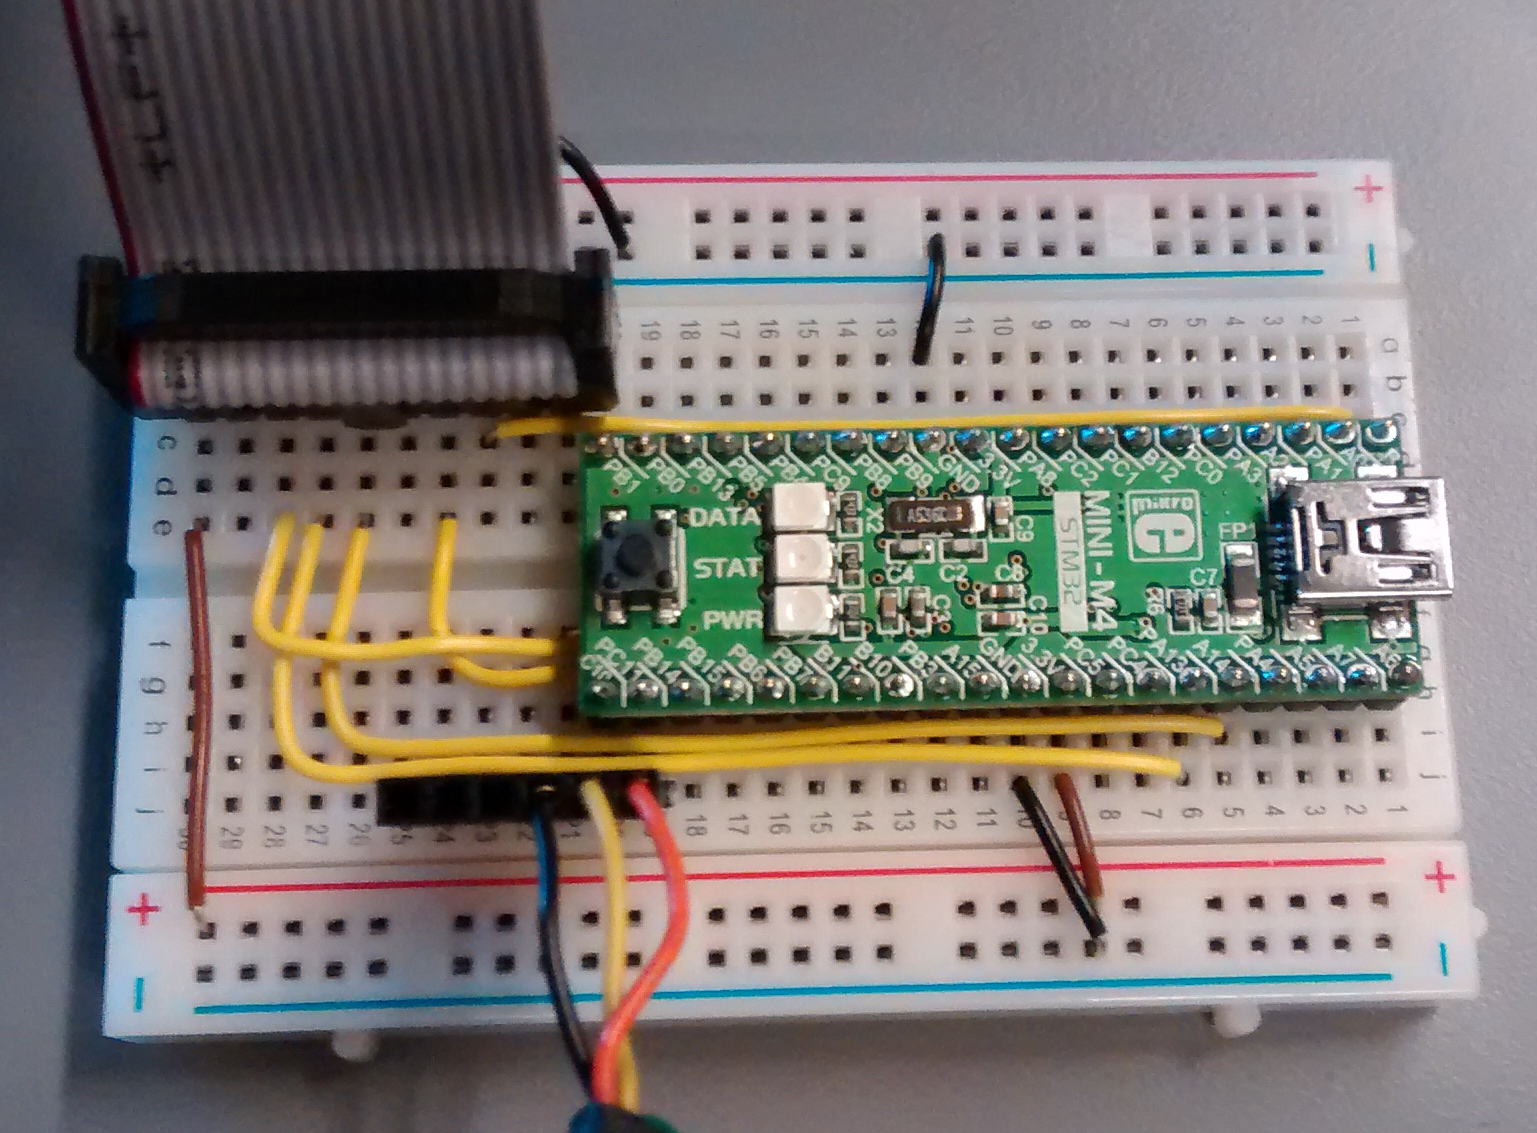
\includegraphics[width=.4\linewidth]{hardware/board_with_jtag_and_serial}
  \caption{Both the JTAG and serial interfaces}
  \label{fig:sub2}
\end{subfigure}
\caption{Connecting the board}
\label{fig:photo2}
\end{figure}

After this, the board was ready to be used in the development process.
The only drawback of this setup, is that it requires three USB ports:
power for the board, the JTAG interface, and the serial communication.

\subsection{JTAG Interface}
\label{ssec:JTAG_Interface}
Figure \ref{fig:sub1} represents the physical layout of the JTAG interface.
Since the JTAG connector has 20 pins, and only some of these are required
to communicate with the board, the set up process took some time to figure
out. The following diagram, shows the pinout of the JTAG and the 
corresponding pins on the microcontroller\textquotesingle s JTAG port.

\begin{figure}[H]
\centering
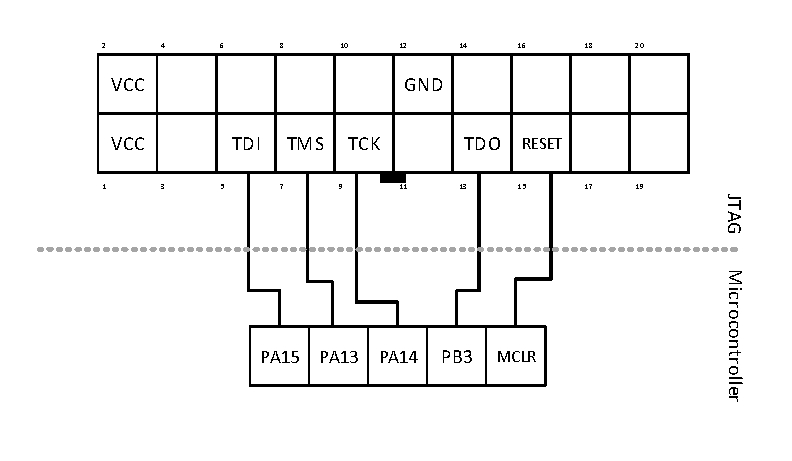
\includegraphics[width=\linewidth,keepaspectratio]{jtag_interface.pdf}
\captionof{figure}{The connection of the JTAG interface}
\label{fig:jtag_interface}
\end{figure}

The tags on the upper part of figure \ref{fig:jtag_interface}, are
JTAG specific:
\begin{labeling}{RESET}
	\item [\textbf{TDI}]
		Test Data In pin
	\item [\textbf{TMS}]
		Test Mode State pin
	\item [\textbf{TCK}]
		Test Clock pin
	\item [\textbf{TDO}]
		Test Data Out pin
	\item [\textbf{RESET}]
		used for resetting the target device. This is connected to the 
		MCLR (Master Clear or Reset) pin of the board
\end{labeling}

The tags on the lower part of the figure represent the pins of the 
microcontroller, where 'P' stand for port, 'A' or 'B' for the port
identity (PORTA) and the number is the individual GPIO needed.

A driver is needed to be installed on Windows machines, in order to
recognize and program using STLINK/v2.
\todo{What about LINUX} 


\section{Source Structure}
The following sections describes different aspects the software used and
the source code located in the project root directory (ESS7\_project) denoted as `/'.
Below the root folder,
all the source code and compiled binaries are roughly structured as listed
in figure \ref{fig:source_structure}:

\begin{figure}[H]
	\dirtree{%
.1 /.
	.2 build.
		.3 ....
	.2 src.
		.3 drivers.
			.4 ....
		.3 kernel.
			.4 ....
		.3 partitions.
			.4 ....
			.4 utils.
	.2 third\_party.
		.3 ARINC.
			.4 APEX.
				.5 ....
		.3 CMSIS.
			.4 ....
		.3 linker\_scripts.
		.3 STM32F4xx\_HAL\_Driver.
			.4 ....
	.2 ....
	}
	\caption{A rough depiction of the source file structure.}
	\label{fig:source_structure}
\end{figure}


\section{Toolchain}
To write, compile and load code to the embedded platform,
a regular computer is used with ones editor of choice,
a C compiler and a programmer unit to transmit the code by the JTAG interface (\ref{ssec:JTAG_Interface}).
The toolchain is adopted from AAURacing\cite{aauracing} which uses a similar chip and develop on Linux\/OSX.
For this project the toolchain has been generalized to also work in windows 10 (later edition?).
In the rest of the section the toolchain and source code(one or two words?) structure is explained.

\subsection{CMAKE}
\label{ssec:cmake}
CMake is used to setup construct the makefiles for the project.
It's of little benefit comparing to write the makefiles from scratch,
but has been adopted in (this OS), since it came with the toolchain.

\begin{displayquote}
CMake is an open-source, cross-platform family of tools designed to build,
test and package software.
CMake is used to control the software compilation process
using simple platform and compiler independent configuration files,
and generate native makefiles and workspaces
that can be used in the compiler environment of your choice\cite{cmake}.
\end{displayquote}

Like Make, CMake is run from a file containing a set instructions on a project.
The instructions can be seperated in a nested structure of files to contain complexity (can you say that?).
A project can have multiple CMake files,
they all have to be named CMakeLists.txt and hence are placed in seperate folders.
The main CMake file is placed in the root-folder of the project and contains the main compiler information.
Specific information about compile targets and their files
are placed in sub files in folders as depicted in figure \ref{fig:cmake_files}.

\begin{figure}[H]
	\dirtree{%
.1 /.
	.2 src.
		.3 CMakeLists.txt.
	.2 third\_party.
		.3 CMakeLists.txt.
	.2 CMakeLists.txt.
	}
	\caption{Placement of CMakeLists.txt files in source directory.}
	\label{fig:cmake_files}
\end{figure}

As denoted by the first line of the CMakeLists.txt file in `/', no less than version 2.8.8 of CMake is required.
The rest of the file set up:

\begin{itemize}
	\item the compiler to use
	\item a list of compiler flags (section \ref{sssec:compiler_flags})
	\item commonly used include paths
	\item two required defines (section \ref{ssec:gcc})
	\item a command to flash the target device using OpenOCD (section \ref{ssec:openocd})
\end{itemize}

Using CMake followed by Make results in a tree of makefiles and objects,
which can be contained by running CMake and Make from within a build folder.
A complete tutorial on how to get started using the build system can be found in Appendix \ref{app:tutorial}.

Make is a UNIX tool\cite{gnu_make} often used to order many calls to GCC in C language projects.
Objects are compiled in separate calls to GCC and
Make provides features to set up a dependency tree of calls when many objects are linked together in a target.

\subsection{GCC}
\label{ssec:gcc}
The GNU Compiler Collection or GCC is used for compiling and linking the C files into a target called `OS'.
Compiling to the ARM architecture a cross compiled version of GCC is necessary,
in this case the arm-none-eabi-gcc compiler which is available in all never Ubuntu versions\cite{arm_gcc}.

\subsubsection{Compiler Flags}
\label{sssec:compiler_flags}
The compiler relies on a list of flags to compile the code to the programmers liking.
The sub section will cover the necessary or otherwise important flags for compiling the (OS).
The entries table \ref{tab:gcc_flags} can be found in the main CMakeLists.txt as referred to in section \ref{ssec:cmake}.

\begin{table}[H]
	\centering
	\begin{tabular}{|c|p{10cm}|}
		\multicolumn{2}{c}{\textbf{MCU flags}} \\
		\multicolumn{2}{c}{These options can be found at gcc.gnu.org \cite{gcc_arm_options}.} \\
		\hline
		-mcpu=cortex-m4   &
		This specifies the name of the target ARM processor. \\
		\hline
		-mtune=cortex-m4  &
		This option specifies the name of the target ARM processor for which GCC should tune the performance of the code. \\
		\hline
		-mthumb           &
		Generate code that executes in Thumb state. \\
		\hline
		-mlittle-endian   &
		Generate code for a processor running in little-endian mode. \\
		\hline
		-mfpu=fpv4-sp-d16 &
		This specifies what floating-point hardware is available on the target. \\
		\hline
		-mfloat-abi=hard  &
		Specifies which floating-point ABI to use.
		`hard' allows generation of FPU-specific floating-point instructions. \\
		\hline
		-mthumb-interwork &
		Generate code that supports calling between the ARM and Thumb instruction sets. \\
		
		\hline
		\multicolumn{2}{c}{} \\
		\multicolumn{2}{c}{\textbf{Linker flags}} \\
		\multicolumn{2}{c}{These options can be found at gcc.gnu.org \cite{gcc_linking_options}.} \\
		\hline
		-Wl, -T.../file.ld &
		Use the linker-script STM32F415RG\_FLASH.ld in the folder
		/third\_party/linker\_scipts (section \ref{ssec:linker_script}). \\
		\hline
		-nostartfiles   &
		Do not use the standard system startup files when linking.
		Used to force GCC to use a custom implementation of Newlibc implemented functions. \\
		\hline
		-Map=./result.map &
		Print a link map to the file result.map showing where object files and symbols are mapped into memory. \\
		
		\hline
		\multicolumn{2}{c}{} \\
		\multicolumn{2}{c}{\textbf{Debugging flags}} \\
		\multicolumn{2}{c}{These options can be found at gcc.gnu.org \cite{gcc_debug_options}.} \\
		\hline
		-g &
		Produce debugging information. \\
		\hline
		-ggdb &
		Produce debugging information for use by GDB. \\
		
		\hline
		\multicolumn{2}{c}{} \\
		\multicolumn{2}{c}{\textbf{C flags}} \\
		\multicolumn{2}{c}{These options can be found at gcc.gnu.org \cite{gcc_c_dialects}.} \\
		\hline
		-std=c99 &
		Determine the language standard to be ISO C99. \\
		\hline
		-fms-extensions &
		Accept some non-standard constructs, useful in some static structures (section ref). \\
		\hline
	\end{tabular}
	\caption{Showing the important GCC flags used to compile the OS.}
	\label{tab:gcc_flags}
\end{table}

There are two important flags, which haven't been mentioned in table \ref{tab:gcc_flags}.
the \texttt{-DHSE\_VALUE=16000000} and \texttt{-DSTM32F415xx} aren't compiler options but definitions passed to GCC to use at compile-time.

\texttt{-DHSE\_VALUE=16000000} defines the value of the external oscillator in hertz.
Specifically it defines \texttt{HSE\_VALUE} to be 16 million hertz as is specified in \cite{hse_value}.
The input of the external oscillator is used as the source for the main clock (some ref to clock setup?).

\texttt{-DSTM32F415xx} simply adds \texttt{STM32F415xx} as a definition at compile-time.
It's used by the HAL library to determine which processor to set up for.

\subsubsection{Linker Script}
\label{ssec:linker_script}
A linker script is used by the compiler to determine where to place different sections of the compiled binary.
Because of this, everything in the output binary gets an offset that matches the memory layout described in section \ref{sec:memory_map}.
The file \texttt{result.map} (table \ref{tab:gcc_flags}) can be used post compilation to determine the location of all symbols in the binary,
as a way to debug the linker-script.\\

The linker-file STM32F415RG\_FLASH.ld is part of the toolchain and is simple to edit to fit any member of the STM32F4 family.
In this project the only necessary change is the definition of flash to be 1MB of size.
Beyond that, the changes depends on the partition requirements on the system.\\

Listing \ref{linker_mem_overview} shows how the memory layout is defined in the linkerscript.
While \texttt{FLASH}, \texttt{RAM} and \texttt{CCMRAM} defines mappings of memory in hardware (see section \ref{sec:memory_map}),
\texttt{OS}, \texttt{DUMMY1}, \texttt{DUMMY2} and \texttt{STDIO\_SYS} defines the location and sizes of the system memory.
In listing \ref{linker_mem_overview}, \texttt{ORIGIN} denotes the starting address of a section of memmory
and \texttt{LENGTH} denotes the size of the section.\\

\begin{minipage}{\linewidth}
\begin{lstlisting}[
	firstnumber=40,
	label=linker_mem_overview,
	caption=\textit{third\_party/linker\_scripts/STM32F415RG\_FLASH.ld}]
/* Specify the memory areas */
MEMORY
{
  FLASH (rx)     : ORIGIN = 0x08000000, LENGTH = 1024K
  OS (rx)        : ORIGIN = 0x08000000, LENGTH =   64K
  DUMMY1 (rx)    : ORIGIN = 0x08010000, LENGTH =    8K
  DUMMY2 (rx)    : ORIGIN = 0x08012000, LENGTH =    8K
  STDIO_SYS (rx) : ORIGIN = 0x08014000, LENGTH =    8K
  RAM (xrw)      : ORIGIN = 0x20000000, LENGTH =  128K
  CCMRAM (rw)    : ORIGIN = 0x10000000, LENGTH =   64K
}
\end{lstlisting}
\end{minipage}

By default all symbols and associated memory goes into the \texttt{OS},
Only when a partition is specifically defined to a location in the linker-script,
can it be seperated from the OS.
Listing \ref{linker_example} shows how to allocate a specific partition.
The linker-script uses the fact that every partition is compiled as a library,
and the library name is added in the listed format under its corresponding label
(in this example: \texttt{STDIO\_SYS}).
This scheme insures the code is separated from the kernel in flash.
It does not, however, separate the statically allocated variables and structures in RAM.\\

\begin{minipage}{\linewidth}
\begin{lstlisting}[
	firstnumber=77,
	label=linker_example,
	caption=\textit{third\_party/linker\_scripts/STM32F415RG\_FLASH.ld}]
.stdio_sys :
{
  . = ALIGN(4);
  libstdio_sys.a:*
  . = ALIGN(4);
} >STDIO_SYS
\end{lstlisting}
\end{minipage}

Simular to listing \ref{linker_example},
the other partitions compiled libraries are confined to a space in flash,
as defined by their labels in \ref{linker_mem_overview}.

\subsection{OpenOCD}
\label{ssec:openocd}
Open On-Chip Debugger or OpenOCD \cite{openocd} is used together with the (hardware goes here) to program the chip and create a channel for GDB to debug the system on-chip.
The CMakeLists.txt file in project root defines a function running the following commands using OpenOCD:

\begin{itemize}
	\item \texttt{init} - Initialize connection
	\item \texttt{reset halt} - Reset and halt the system
	\item \texttt{flash write\_image erase \$\{elf\_file\}} - Write binary image to chip
	\item \texttt{reset run} - Reset chip and start normal execution
\end{itemize}

Above, \texttt{\$\{elf\_file\}} is the compiled output binary.

After execution of this command, OpenOCD will remain open and connected to the
chip and it will accept incoming connections on port 3333 for
GDB debugging as a GDB server (see more in \ref{ssec:gdb}.

\subsection{GDB}
\label{ssec:gdb}
\todo{Write GDB version}
The GNU Project debugger\cite{gdb}, GDB, is an open source software debugger
built to compliment the GNU Project compilers, GCC (see \ref{ssec:gcc}). It
allows programmers to more intelligently debug their applications.
GDB can\\
\begin{itemize}
	\item attach to a remote program, even running on a different piece of
	hardware. 
	\item pause execution of a program at specified lines of code with
	breakpoints.
	\item show the content of memory, either by direct a addressing or by
	variable name.
	\item if the hardware supports it, show the value of each CPU register.
	\item execute code line by line, letting the programmer see how each line
	affects the state of the program, and in case of crashing code, which line
	of code crashes the program.
\end{itemize}
This feature set, makes GDB especially useful for tracking down complex bugs and
bugs in otherwise inaccessible systems, e.g. systems with no screen to directly 
print to. GDB also allows programmers to investigate buggy code while it is
running, as opposed to after-the-fact debugging of logging, printing, etc.
Many advanced text editors and integrated development environments feature
direct seamless GDB integration. Outside of such programs, GDB can be run in 
command line.

To debug the code running on the chip, an active OpenOCD connection to the chip
is required. When OpenOCD is connected, it will act as a GDB server. GDB can
be connected to OpenOCD with the command \texttt{target remote localhost:3333}.

\section{Drivers}

Setting up the drivers took place in the beginning of the project. Their
functionality rely a lot on the HAL library. Even though the process is
quite straightforward, there is some learning involved in how to use the
library. The library\textquotesingle s documentation is a good starting
point, and the things it lacks can be found in the 
microcontroller\textquotesingle s datasheet.

\subsection{System clock}
The initial setting for the clock is that it uses the internal oscillator,
which runs at 16MHz. In order to get the maximum speed supported by the
CPU, the board needs to be configured to multiply this frequency.
However, instead of using the internal oscillator which can be imprecise, 
the Mini-M4 
board has an external oscillator\footnote{Featuring less wander (slow
 variations due to temperature and aging) and jitter(fast variations)} 
that can be used as the main clock 
source. This is represented in figure \ref{fig:system_clock} with the HSE
tag. These tags refer to the location and the speed of the oscillators
present on the board or inside the microcontroller:

\begin{labeling}{HSE}
	\item[\textbf{HSE}]
		high-speed external oscillator, the main clock source
	\item[\textbf{HSI}]
		high-speed internal oscillator, not used
	\item[\textbf{LSE}]
		low-speed external oscillator, used by the real-time clock
	\item[\textbf{LSI}]
		low-speed internal oscillaror, used by the independent watchdog
		timer
\end{labeling}

\begin{figure}[H]
\centering
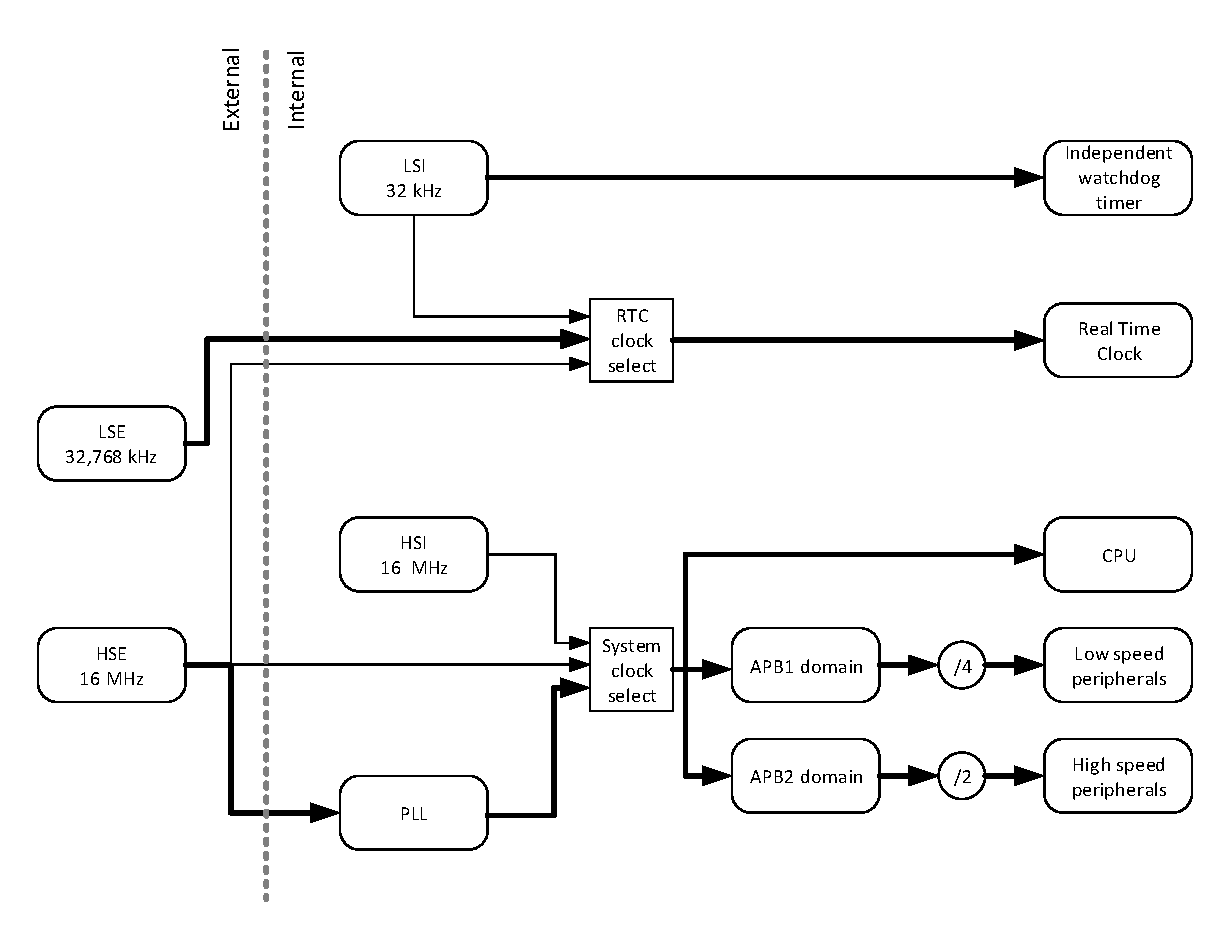
\includegraphics[width=\textwidth]{system_clock.pdf}
\caption{An advanced system overview}
\label{fig:system_clock}
\end{figure}

The lower part of figure \ref{fig:system_clock} shows that the frequency
of the HSE is multiplied by a PLL(Phase-locked loop) system, before it gets
to the clock selection block. After this, the frequency is supplied to
the CPU bus, and scaled down for the peripheral busses. The latter are
divided into low and high speed domains as:

\begin{labeling}{APB1 domain}
	\item[\textbf{APB1 domain}]
		low-speed domain, running at 42 Mhz. This includes among other 
		peripherals the UART.
		
	\item[\textbf{APB2 domain}]
		high-speed domain, running at 84 mHz.
	\end{labeling}

\subsection{UART}

\todo[inline,color=green]{
The UART sets the speed of the transmission and reception of the information between the STM32 and the outside. The communication is made by one character at a time. The transmission is activated by the interrupts and it can happen both ways simultaneously, or one way at a time. An UART has a clock generator, that we set for 16Mz, input and output registers, transmit/receive control, read/write control logic, and transmit/receiver buffers.
It is also possible to communicate with the UART using a screen, getting some important output for debugging.}

\subsection{LEDs}

\subsection{Delay}

\subsection{MPU}

\subsection{Timing function}
This driver is used for precise measuring the execution time of different functions. It uses the DWT
 registers defined in the ARM-M4 Architecture manual. These are responsible for Data Watchpoint 
 and Trace support. By using one of these counters, one could follow the system's clock ticks. 
 At a core frequency of 168 MHz, each tick would take 5.45 nanoseconds.\\
In order to do this, the DWT\textunderscore CONTROL register is set to a value that allows the system's clock to be sent to DWT\textunderscore CYCCNT. After this, the time can easily be tracked by converting the value of DWT\textunderscore CYCCNT.

\subsection{Watchdog timer}
% \ http://electronics.stackexchange.com/questions/123080/independent-watchdog-iwdg-or-window-watchdog-wwdg
The STM32 MCU has two watchdog timers ready to reset the program, in case of an error.
The first one, is the independent watchdog timer, based on an independent oscillator (32 kHz).
When initialised, the watchdog timer receives a value, from which it starts counting down, using
the ticks from the crystal. In the meanwhile, the program has to reset this count, by refreshing 
the timer to the same value it used before. If this fails to happen, when the count reaches zero, 
the watchdog timer will react by restarting the board.
\\
The second watchdog timer, is called a window watchdog. In contrast to the independent watchdog, 
one can provide a time interval in which the timer has to be reset. Resetting the timer outside this interval(as well as not resetting it in the mentioned time window) would restart the program. It uses 
the system clock, which means that if this fails, the watchdog won't be able to reset the system.

\subsubsection{Specifics}
The driver for the independent watchdog works by setting a prescaler on the 32kHz crystal to match 
the time requirements of the program(multiples of milliseconds). The watchdog is then initialised 
and started using the HAL library specific functions. \\
When the program is run, the watchdog restarts it after the interval of time set in the initialisation
phase runs out. In order to have the program running as usual, the refresh function has to be called,
 at intervals shorter than the initial time span.

\subsection{RTC}

\section{System Calls}
\todo[inline,color=green]{needs to be moved}
System calls are implemented with the ARMv7M instruction \texttt{SVC} (Supervisor
Call). When this instruction is executed, a interrupt will be triggered. Already
set up by the CMSIS library, any SVC interrupts will trap into the function
named \texttt{SVC\_Handler}.
In order to avoid having to deal with assembly\footnote{It is necessary to use
assembly code to issue an \texttt{SVC} instruction} code in partition level
software, system call functions (including the APEX functions) are implemented
as a library that entirely handles the system call.
The sequence of steps for making a system call is a follows:\\

\begin{tabular}{ r l p{10.5cm} }
    1. & Userspace & Partition code calls one of the system call wrapper
    functions.\\
    2. & Userspace & The wrapper function moves the number denoting the system
    call function into register R0.\\
    3. & Userspace & The wrapper function moves any input arguments into the
    registers R1-R3 and R12. If the function has more than four input arguments,
    those must be stacked.\\
    4. & Userspace & The wrapper function issues an \texttt{SVC} instruction.\\
    5. & Hardware & The NVIC stacks the registers R0-R3, R12, PC and LR and
    branches to the \texttt{SVC\_Handler} function.\\
    6. & Kernelspace & The \texttt{SVC\_Handler} function investigates the
    stacked value of register R0 to determine which function the partition level
    code wished to execute.\\
    7. & Kernelspace & The \texttt{SVC\_Handler} function calls the appropriate
    function with the input arguments from the stacked registers.\\
    8. & Kernelspace & The \texttt{SVC\_Handler} puts the results of the
    function in the stacked registers. The return code is moved to R0, and
    additional output is put in the registers R1-R3 and R12. If necessary, more
    output is put in the stack.\\
    9. & Kernelspace & The \texttt{SVC\_Handler} returns.\\
    10. & Hardware & The NVIC restores the registers R0-R3, R12, PC and LR from
    the stack and returns execution to the system call wrapper function.\\
    11. & Userspace & The wrapper function returns the output from the system
    call as stored in the registers to the calling partition code.\\
\end{tabular}\\


Only the registers R0-R3 and R12 are available for argument passing, as these
are the only general purpose registers that are stacked by the NVIC. The NVIC
does not clear the registers before entering the \texttt{SVC\_Handler} function,
and thus all the general purpose registers may contain the same values as when
the \texttt{SVC} instruction was executed, but their consistency is not
garantued, as other interrupt service routines could have run before the
\texttt{SVC\_Handler} function started execution.\\
To avoid rescheduling occuring during a system call, the SysTick interrupt is
turned off during the execution of the \texttt{SVC\_Handler} function.\\
Each system call is identified by the number the caller has moved into the R0
register before issuing the \texttt{SVC} instruction. The \texttt{SVC}
instruction does supply a way to embed this number directly as a part of the
instruction as an immediate value, instead of using a seperate register, but
dedicating a register to this was chosen for two reason: One, it is poorly
documented how software can read the value embedded in the instruction, and two,
to keep it consistent with how system calls are handled on other architectures
such as x86.\\
Table \ref{tab:syscalls} shows all the implemented system calls and their
identifier.

\begin{table}
\centering
	\begin{tabular}{| l | l |}
		\hline
		Identifier		&	Name \\
		\hline
		0xC0FFEE0A		&	CREATE\_PROCESS 			\\
		\hline
		0xC0FFEE0B		&	GET\_TIME					\\
		\hline
		0xC0FFEE0C		&	CREATE\_QUEUING\_PORT 		\\
		\hline
		0xC0FFEE0D		&	RECEIVE\_QUEUING\_PORT 		\\
		\hline
		0xC0FFEE0E		&	SEND\_QUEUING\_PORT 		\\
		\hline
		0xC0FFEE0F		&	GET\_QUEUING\_PORT\_ID 		\\
		\hline
		0xC0FFEE10		&	GET\_QUEUING\_PORT\_STATUS	\\
		\hline
		0xC0FFEE11		&	PROCESS\_STOP\_SELF 		\\
		\hline		
	\end{tabular}
\caption{A table of the implemented system calls and their identifier.}
\label{tab:syscalls}
\end{table}

\section{XML configuration file}
\todo{Write about the manual writing of the XML config file?}

\subsection{XML Parser}

The configuration of the OS is not usable in its XML format. open653 is written in C; therefore a dynamic parser written in Python has been created to generate C structs from the XML.
\todo{reference for xmltodict}
Using an external library xmltodict.py, the XML is converted into a JSON structure which makes navigating and accessing sub nodes very easy as it becomes a nested dictionary structure with lists.
The generation of the structs is handled as two seperate file writes. xml\_data.h is mostly statically defined as it contains the declarations for the C structs. The majority of the content of that file is read and re-written into the file from another file called xml\_data\_template.h. The rest of the file is written dynamically from the configuration data as references to its content.
xml\_data.c is fully dynamic and generated from the elements in the XML. The four major elements (partitions, partition\_memory, module\_schedule and connection\_table) are looped through, populating formatted strings, and then are written to the file.

\subsection{C Structures}

\section{OS}

\subsection{Init\/main}

\subsubsection{MPU Setup}
\subsubsection{Partition Setup}
\subsubsection{Process Setup}

\subsection{Scheduling}

\subsubsection{SysTick}

\subsubsection{Context Switching}
There are multiple different states the processor can be in, when a context 
switch from one process to another occurs. The state determines whether the
Master Stack Pointer or the Process Stack Pointer was used by the process,
and whether the FPU was used by the process or not. Because of this, the context
switch algorithm must start by determining the processor state in order to know
which registers
to save and where to save them to.\\
The processor state is saved in the Link return register, and it can be one of
the possible six EXC\_RETURN values (see figure \ref{tab:exc-return}).\\
If the pre-empted process used the FPU, the FPU registers S16 to S31
should also be saved by software in addition to the general purpose regisers.
Because of time constraint, this was not implemented.\\
The registers are saved entirely on the stack. Therefore, it is important for
the software to know which
stack pointer to use when saving the remaining registers. So the very first
thing the interrupt service routine (ISR) used for scheduling must do, is to inspect
the \excreturn\ value in the LR register to determine wether to use the 
Master Stack Pointer or the Process Stack Pointer. The software must then, at 
the address denoted by the stack pointer, save the registers that have yet to be
saved, and update the stack pointer, before saving both the stack pointer and
the \excreturn\ value to the process structure elsewhere in memory. This is all
done in assembly to make sure that there is complete control over which
registers are used, so as to avoid overwriting any registers that have yet to be
saved. This is absolutely necessary, as otherwise the state of register for a
process might be corrupted during a context switch. Additionally, any ISR used
for scheduling must be declared as naked\footnote{A naked function has no
compiler generated prologue and epilogue. This means that the compiler does not
save any registers on the stack before using them, and it does not restore them
before ending a function.}, to avoid the compiler changing registers before the
context can be saved, and to give complete control over which value is pushed to
the PC register at the end of the ISR.\\
After the context has been saved, control is handed over to the scheduler, which
can then decide which process should be running next.\\
Once all the operations the ISR has completed, the context of the process
selected by the scheduler must be restored. From this point, the code must once
again be written in assembly to avoid overwriting a register after it has been 
restored. First, the registers saved by software on the stack must be restored,
then based on the \excreturn\ value the process interrupted with, it can be 
determined to which stack pointer register the new stack pointer must be pushed
to. Lastly, execution must return to the process by pushing the \excreturn\ value
to the PC register. The \excreturn\ value pushed to the PC register must be the
same as that read from the LR register when the process was interrupted.
Figure \ref{fig:flowchart_contextswitch}\todo{Write caption for this figure.} shows the flow when switching contexts.
\begin{figure}
    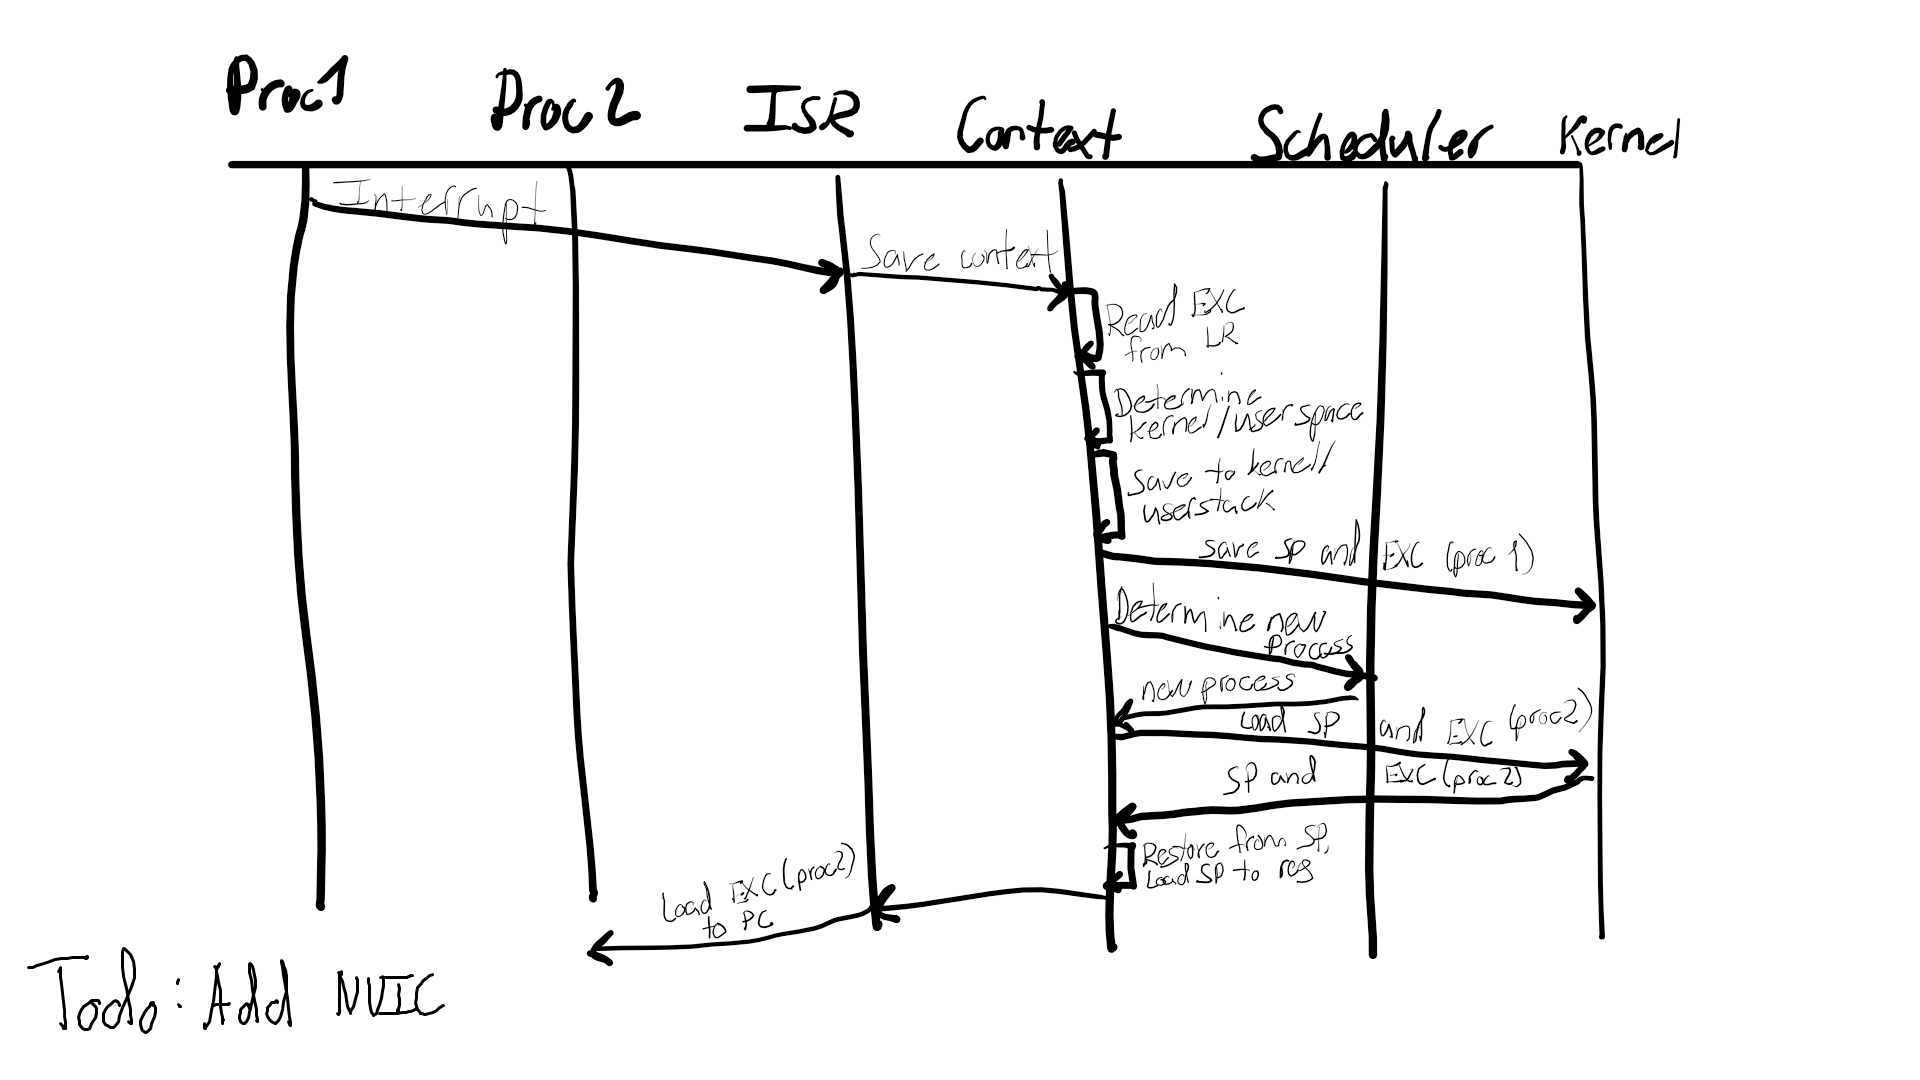
\includegraphics[width=\textwidth]{figures/flowchart_contextswitch.png}
    \caption{This is just a placeholder.}
    \label{fig:flowchart_contextswitch}
\end{figure}

\subsubsection{windows}

\subsubsection{Partition Scheduler}

\subsubsection{Process scheduler}


\subsection{Ports}

\subsubsection{Queuing Ports}
\subsubsection{Sampling Ports}


\subsection{APEX}

\subsubsection{Syscalls}


\subsection{Error Handling}


\section{Partitions and processes}

\subsection{Partitions}

\subsection{Processes}

\subsection{idle\_sys}

\subsection{stdio\_sys}

\subsection{dummy1}

\subsection{dummy2}

\subsection{evil}


\section{Features of the system}
\todo[inline, color=green]{Here we can have a table showing what features
our system has, what features were not implemented, in regards to the
standard}
